\documentclass{article}
\usepackage[margin=1in]{geometry}
\usepackage{amsmath}
\usepackage{amssymb}
\usepackage{pgfplots}
\usepgfplotslibrary{units}
\pgfplotsset{width=9cm, compat=1.9}

\begin{document}

\title{Calculus 1 Study Guide and Notes}
\date{}
\author{Written by David Corbin\\ \small{Based on James Stewart Calculus Eighth Edition}}
\maketitle

%
% Chapter 1.1
%

\section*{1.1 Representing Functions}

A function \(f\) is a rule that assigns to each element \(x\) in set \(D\) exactly one element, called \(f(x)\), in a set \(E\).\\

Vertical Line Test: A curve in the \(xy\)-plane is the graph of a function of \(x\) if and only if no vertical line intersects the curve more than once.\\

A piecewise function is a function defined for multiple sub-functions applying to a certain intergal of the main function's domain.\\


\[ f(x)=
    \begin{cases} 
      1-x & x\leq -1 \\
      \frac{3-x}{4} & -1 < x < 100 \\
      2x & x\geq 100
   \end{cases}
\]\\

A function is even if \(f(-x)=f(x)\) for every number \(x\) in its domain.\\

A function is odd if \(f(-x)=-f(x)\) for every number \(x\) in its domain.\\

A function \(f\) is decreasing on an interval \(I\) if \(f(x_1)<f(x_2)\) whenever \(x_1 < x_2\) in \(I\).

A function \(f\) is increasing on \(I\) if \(f(x_1)>f(x_2)\) whenever \(x_1<x_2\) in \(I\).\\
%
% Chapter 1.2
%

\section*{1.2 Types of Functions}

A linear function can be written in \textbf{slope-intercept form} (\(y=mx+b\)) where \(m\) is the slope of the line and \(b\) is the y-intercept.
\\\\
A function \(P\) is a \textbf{polynomial} if 
$$P(x)=a_n{x}^n+a_{n-1}x^{n-1}+ \cdots +a_2x^2+a_1x+a_0$$
where n is a non-negative integer and the numbers \(a_0, a_1, a_2, \ldots ,a_n\) are constants called the \textbf{coefficients} of the polynomial. The domain of any polynomial is \(\mathbb{R} = (-\infty, \infty)\). If the coefficient \(a_n \neq 0\), then the degree of the polynomial is \(n\).
\\\\
A polynomial of degree 2 is of the form \(P(x)=ax^2+bx+c\) and is called a \textbf{quadratic function}. Its graph is always a parabola that opens upward if \(a > 0\) and downward if \(a < 0\).
\\\\
A polynomial of degree 3 is of the form 
\[ P(x)=ax^3+bx^2+cx+d \text{ where } a \neq 0 \]
and is called a \textbf{cubic function}.
\\\\
A function of the form \(f(x) = x^a\), where \(a\) is a constant, is called a \textbf{power function}.
\\\\
A \textbf{rational function} \(f\) is a ratio of two polynomials:
\[ f(x)=\frac{P(x)}{Q(x)} \]
where \(P\) and \(Q\) are polynomials. The domain consists of all \(x\)-values such that \( Q(x) \neq 0 \).

\subsection*{Graphs of Basic Trigometric Functions}

\begin{center}
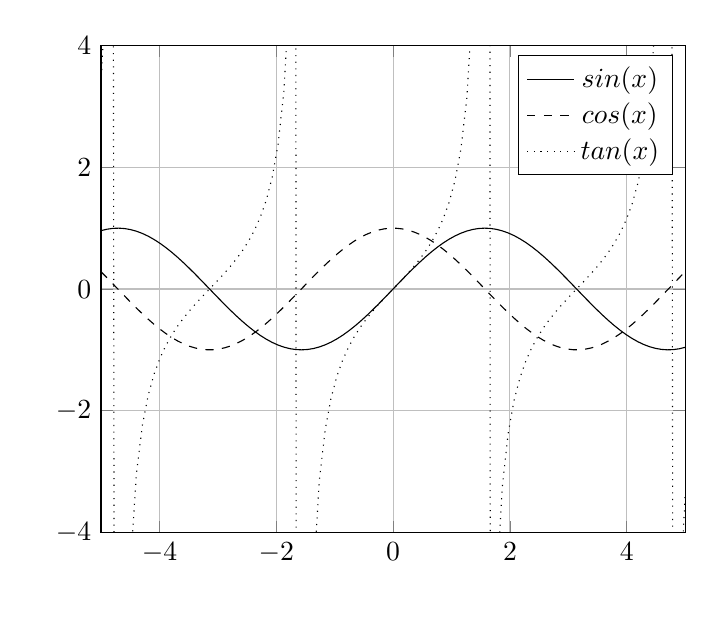
\begin{tikzpicture}
\begin{axis}[
    %axis lines = bottom,
    grid=both,
    ymin=-4,
    ymax=4,
    xmax=5,
    xmin=-5
]

% Sine function
\addplot [
    domain=-5:5,
    samples=100
]
{sin(deg(x))};
\addlegendentry{$sin(x)$}

% Cosine function
\addplot [
    domain=-5:5, 
    samples=100,
    dashed
]
{cos(deg(x))};
\addlegendentry{$cos(x)$}


% Cosine function
\addplot [
    domain=-5:5, 
    samples=100,
    dotted
]
{tan(deg(x))};
\addlegendentry{$tan(x)$}

 
\end{axis}
\end{tikzpicture}
\end{center}
Notice that for both sine and cosine functions the domain is \((-\infty, \infty)\) and the range is the closed interval \([-1, 1]\). In addition, sine and cosine functions are periodic functions with a period of 2\(\pi\). 
$$\sin(x+2\pi)=\sin(x) \quad \quad \cos(x+2\pi)=\cos(x)$$
\textbf{Exponential functions} are functions of the form \(f(x)=b^x\) where the base \(b\) is a positive constant.
\\\\
\textbf{Logarithmic functions} are functions written as \(f(x)=\log_b(x)\), where the base \(b\) is a positive constant, are the inverse functions of exponential functions.

%
% Chapter 1.3
%

\section{More advanced functions}

Vertical and Horizontal Shifts\\

Suppose \(c>0\). Then
\begin{center}
\(y=f(x)+c\) is the graph of \(y=f(x)\) shifted \(c\) units upward.\\
\(y=f(x)-c\) is the graph of \(y=f(x)\) shifted \(c\) units downward.\\
\(y=f(x+c)\) is the graph of \(y=f(x)\) shifted \(c\) units to the left.\\
\(y=f(x-c)\) is the graph of \(y=f(x)\) shifted \(c\) units to the right.\\
\end{center}
Vertical and Horizontal Stretching and Reflecting\\

Suppose \(c>1\). Then
\begin{center}
\(y=cf(x)\) is the graph of \(y=f(x)\) stretched vertically by a factor of \(c\).\\
\(y=(1/c)f(x)\) is the graph of \(y=f(x)\) shrunk vertically by a factor of \(c\).\\
\(y=f(cx)\) is the graph of \(y=f(x)\) shrunk horizontally by a factor of \(c\).\\
\(y=f(x/c)\) is the graph of \(y=f(x)\) stretched horizontally by a factor of \(c\).\\
\(y=-f(x)\) is the graph of \(y=f(x)\) reflected about the \(x\)-axis.\\
\(y=f(-x)\) is the graph of \(y=f(x)\) relected about the \(y\)-axis.
\end{center}

%
% Chapter 1.4
%

\section*{1.4 Tangent and Velocity} 

A \textbf{tangent} is a line touching a curve. A tangent line has the same direction as the curve at the point of contact. A secant line, on the other hand, cuts throught the curve more than once.
\\\\
To find the tangent at a point on a curve (in slope-intercept form: \(y=mx+b\)), we must find the slope \(m\) at that point and use it to find \(b\) (the \(y\)-intercept). 

\subsection*{Average Velocity}

$$\text{average velocity} = \frac{\text{change in position}}{\text{elapsed time}}$$ 

%
% Chapter 1.5
%

\section*{1.5 Limit of a Function}

\subsection*{Limit}

We can make the values of \(f(x)\) arbitrarily close to \(L\) by restricting \(x\) to be sufficiently close to \(a\) but never equal to \(a\).
$$\lim_{x \to a}f(x)=L \text{ means that } f(x) \to L \text{ as } x \to a$$

\subsection*{One-sided Limit}

$$\lim_{x \to a^-}f(x)=L$$
means that the limit of \(f(x)\) as \(x\) approaches \(a\) from the left is equal to \(L\) if we can make the values of \(f(x)\) arbitrarily close to \(L\) by taking \(x\) to be sufficiently close to \(a\) with \(x\) less than \(a\).

$$\lim_{x \to a}f(x)=L \quad \text{if} \quad \lim_{x \to a^-}f(x)=L \quad \text{and} \quad \lim_{x \to a^+}f(x)=L$$

\subsection*{Infinite Limits}

Let \(f\) be a function defined on both side of \(a\), except possibly at \(a\) itself. Then 
$$\lim_{x \to a}f(x)=\infty$$
means that the values of \(f(x)\) can be made arbitrarily large by taking \(x\) sufficiently close to \(a\), but not equal to \(a\).
\\\\
Let \(f\) be a function defined on both side of \(a\), except possibly at \(a\) itself. Then 
$$\lim_{x \to a}f(x)=-\infty$$
means that the values of \(f(x)\) can be made arbitrarily large negative by taking \(x\) sufficiently close to \(a\), but not equal to \(a\).

\subsection*{Vertical Asymptotes}

The line \(x=a\) is called \textbf{vertical asymptote} of the curve \(y=f(x)\) if at least one of the following statements is true:

$$\lim_{x \to a}f(x)=\infty \quad \lim_{x \to a^-}f(x)=\infty \quad \lim_{x \to a^+}f(x)=\infty$$
$$\lim_{x \to a}f(x)=-\infty \quad \lim_{x \to a^-}f(x)=-\infty \quad \lim_{x \to a^+}f(x)=-\infty$$


%
% Chapter 1.6
%

\section*{1.6 Limit Laws}

Suppose that \(c\) is the constant and the limits 
$$\lim_{x-a}f(x) \quad \text{ and } \quad \lim_{x \to a}g(x)$$
exist. Then
$$\textbf{1. }\lim_{x \to a}[f(x)+g(x)]=\lim_{x \to a}f(x) + \lim_{x \to a}g(x)$$
$$\textbf{2. }\lim_{x \to a}[f(x)-g(x)]=\lim_{x \to a}f(x) - \lim_{x \to a}g(x)$$
$$\textbf{3. }\lim_{x \to a}[cf(x)]=c\lim_{x \to a}f(x)$$
$$\textbf{4. }\lim_{x \to a}[f(x)g(x)]=\lim_{x \to a}f(x) \times \lim_{x \to a}g(x)$$
$$\textbf{5. }\lim_{x \to a}[\frac{f(x)}{g(x)}]=\frac{\lim_{x \to a}f(x)}{\lim_{x \to a}g(x)} \text{ if } \lim_{x \to a}g(x) \neq 0 $$
$$\textbf{6. }\lim_{x \to a}[f(x)]^n=[\lim_{x \to a}f(x)]^n \text{ where } n \text{ is a postitive integer.}$$
$$\textbf{7. }\lim_{x \to a}c=c$$
$$\textbf{8. }\lim_{x \to a}x=a$$
$$\textbf{9. }\lim_{x \to a}x^n=a^n \text{ where } n \text{ is a positive integer}$$
$$\textbf{10. }\lim_{x \to a}\sqrt[n]x=\sqrt[n]a \text{ where } n \text{ is a positive integer}$$
$$\textbf{11. }\lim_{x \to a}\sqrt[n]{f(x)}=\sqrt[n]{\lim_{x \to a}f(x)} \text{ where } n \text{ is a positive integer}$$

\begin{enumerate}
    \item The limit of the sums is the sum of the limits.
    \item The limit of the difference is the difference of the limits.
    \item The limit of a constant times a function is the constant times the limit of the function.
    \item The limit of the product is the product of the limits.
    \item The limit of the quotient is the quotient of the limits (provided that the limit of the denominator is not 0).
\end{enumerate}

\subsection*{Direct Substitution Property}

If \(f\) is a polynomial or a rational function and \(a\) is in the domain of \(f\), then 
$$\lim_{x \to a}f(x)=f(a)$$

\subsection*{Sequeeze Theorem}

If \(f(x) \leq g(x) \leq h(x)\) when x is near \(a\) (except at \(a\)) and 
$$\lim_{x \to a}f(x)=\lim_{x \to a}h(x) = L$$
then
$$\lim_{x \to a}g(x) = L$$

%
% Chapter 1.7
%

\section*{1.7 Definition of a Limit}

\subsection*{Formal Definition of a Limit}

Let \(f\) be a function defined on some open interval that contains the number \(a\), except possibly \(a\) itself. Then we say that the limit of \(f(x)\) as \(x\) approaches \(a\) is \(L\) and we write
$$\lim_{x \to a}f(x)=L$$
if for every number \(\epsilon > 0\) there is a number \(\delta > 0\) such that
$$\text{if} \quad 0< \left| x-a \right| <\delta \quad \text{then} \quad \left| f(x)-L \right| <\epsilon$$

\subsection*{Formal Definition of a Left-Hand Limit}

$$\lim_{x \to a^-}f(x)=L$$
if for every number \(\epsilon > 0\) there is a number \(\delta > 0\) such that 
$$\text{if} \quad a-\delta<x<a \quad \text{then} \quad \left| f(x)-L \right| <\epsilon$$ 

\subsection*{Formal Definition of a Right-Hand Limit}

$$\lim_{x \to a^+}f(x)=L$$
if for every number \(\epsilon > 0\) there is a number \(\delta > 0\) such that 
$$\text{if} \quad a<x<a+\delta \quad \text{then} \quad \left| f(x)-L \right| <\epsilon$$ 

\subsection*{Formal Definiton of an Infinite Limit}

Let \(f\) be a function defined on some open interval that contains the number \(a\), except \(a\) itself. Then
$$\lim_{x \to a}f(x)=\infty$$

means that for every positive number \(M\) there is a positive number \(\delta\) such that 
$$\text{if} \quad 0< \left| x-a \right| <\delta \quad \text{then} \quad f(x)>M$$


\subsection*{Formal Definiton of a Negative Infinite Limit}

Let \(f\) be a function defined on some open interval that contains the number \(a\), except \(a\) itself. Then
$$\lim_{x \to a}f(x)=-\infty$$
means that for every negative number \(N\) there is a positive number \(\delta\) such that 
$$\text{if} \quad 0< \left| x-a \right| <\delta \quad \text{then} \quad f(x)>N$$


%
% Chapter 1.8
%

\section*{1.8 Continuity}

A function is continuous at a number \(a\) if 
$$\lim_{x \to a}f(x) = f(a)$$\\
A function \(f\) is continuous from the right at a number \(a\) if 
$$\lim_{x \to a^+}f(x)=f(a)$$
and \(f\) is continuous from the left at \(a\) of 
$$\lim_{x \to a^-}f(x)=f(a)$$\\
A function \(f\) is continuous on an interval if it is continuous at every number in the interval.
\\\\
If \(f\) and \(g\) are continuous at \(a\) and if \(c\) is a constant, then the following functions are also continuous at \(a\).
\begin{enumerate}
    \item \(f + g\)
    \item \(f - g\)
    \item \(cf\)
    \item \(fg\)
    \item \(\frac{f}{g}\) if \(g(a) \neq 0\)
\end{enumerate}
Any polynomial, rational function, root function, or trigonometric function is continuous anywhere on its domain.

\subsection*{Intermediate Value Theorem}

Suppose that \(f\) is continuous on the closed interval \([a, b]\) and let \(N\) be any number between \(f(a)\) and \(f(b)\), where \(f(a) \neq f(b)\). Then there exists a number \(c\) in \((a, b)\) such that \(f(c)\) = \(N\).

%
% Chapter 2.1
%

\section*{2.1 Derivative and Rates of Change}

\subsection*{Tangents}

The \textbf{tangent line} to the curve \(y=f(x)\) at the point \(P(a, f(a))\) is the line through \(P\) with slope 
$$m=\lim_{x \to a}\frac{f(x)-f(a)}{x-a} \Leftrightarrow m=\lim_{h \to 0}\frac{f(a+h)-f(a)}{h}$$
as long as the limit exists.

\subsection*{Velocities}

$$\text{average velocity}=\frac{\text{displacement}}{\text{time}}=\frac{f(a+h)-f(a)}{h}$$\\
Instantaneous velocity at time \(t = a\) is defined as 
$$v(a) = \lim_{h \to 0}\frac{f(a+h)-f(a)}{h}$$

\subsection*{Derivatives}

The derivative of a function \(f\) at a number \(a\), denoted by \(f'(a)\), is 
$$f'(a)=\lim_{h \to 0}\frac{f(a+h)-f(a)}{h}$$
if the limit exists.

\subsection*{Rates of Change}

The average rate of change of \(y\) with respect to \(x\) over the interval \([x_1, x_2]\) is the difference quotient
$$\frac{\Delta x}{\Delta y}=\frac{f(x_2)-f(x_1)}{x_2-x_1}$$
\\
The instantaneous rate of change of \(y\) with respect to \(x\) is 
$$\lim_{\Delta x \to 0}\frac{\Delta y}{\Delta x}=\lim_{x_2 \to x_1}\frac{f(x_2)-f(x_1)}{x_2-x_1}$$
The derivative \(f'(a)\) is the instantaneous rate of change of \(y=f(x)\) with respect to \(x\) when \(x=a\).


%
% Chapter 2.2
%

\section*{2.2 Derivatives as Functions}

$$f'(x)=\lim_{h \to 0}\frac{f(x+h)-f(x)}{h}$$
\(f'(x)\) can be interpreted geometrically as the slope of the tangent line to the graph of \(f\) at the point \((x, f(x))\)
\\\\
A function \(f\) is \(\textbf{differentiable}\) at \(a\) if \(f'(a)\) exists. It is differentiable on an open interval \((a,b)\) if it is differnetiable at every number in the interval.
\\\\
If \(f\) is differentiable at \(a\), the \(f\) is continuous at \(a\).

\subsection*{Ways a Function can be Discontinuous}

\begin{enumerate}
    \item corner point
    \item discontinuity
    \item vertical tangent
\end{enumerate}


%
% Chapter 2.3
%

\section*{2.3 Differentiation Formulae}

\begin{enumerate}
    \item \(\frac{d}{dx}(c)=0\) \quad where \(c\) is a constant
    \item \(\frac{d}{dx}(x)=1\)
    \item \(\frac{d}{dx}(x^n)=nx^{n-1}\) \quad if \(n\) is a positive integer
    \item \(\frac{d}{dx}[cf(x)]=c\frac{d}{dx}f(x)\) \quad where \(c\) is a constant and \(f(x)\) is differentiable
    \item \(\frac{d}{dx}[f(x)+g(x)]=\frac{d}{dx}f(x)+\frac{d}{dx}g(x)\) \quad if \(f(x)\) and \(g(x)\) are differentiable
    \item \(\frac{d}{dx}[f(x)-g(x)]=\frac{d}{dx}f(x)-\frac{d}{dx}g(x)\) \quad if \(f(x)\) and \(g(x)\) are differentiable
    \item \(\frac{d}{dx}[f(x)g(x)]=f(x)\frac{d}{dx}[g(x)]+g(x)\frac{d}{dx}[f(x)]\) \quad if \(f\) and \(g\) are differentiable
    \item \(\frac{d}{dx}[\frac{f(x)}{g(x)}]=\frac{g(x)\frac{d}{dx}[f(x)]-f(x)\frac{d}{dx}[g(x)]}{g(x)^2}\) \quad if \(f\) and \(g\) are differentiable
\end{enumerate}
\begin{enumerate}
    \item The derivative of a constant is 0.
    \item The derivative of x is 1.
    \item The general power rule
    \item The derivative of a constant times a function is the constant times the derivative of the function.
    \item The derivative of a sum of functions is the sum of the derivatives.
    \item The derivative of the difference is the difference of the derivatives.
    \item The product rule
    \item The quotient rule
\end{enumerate}

%
% Chapter 2.4
%

\section*{2.4 Derivatives of Trigonometric Functions}

\[ \lim_{\theta \to 0} \frac{\sin(\theta)}{\theta}=1 \]
\[ \lim_{\theta \to 0} \frac{\cos(\theta)-1}{\theta}=0 \]
\[ \frac{d}{dx}(\sin(x))=\cos(x) \]
\[ \frac{d}{dx}(\cos(x))=-\sin(x) \]
\[ \frac{d}{dx}(\tan(x))=\sec^2(x) \]
\[ \frac{d}{dx}(\csc(x))=-\csc(x)\cot(x) \]
\[ \frac{d}{dx}(\sec(x))=\sec(x)\tan(x) \]
\[ \frac{d}{dx}(\cot(x))=-\sec^2(x) \]

%
% Chapter 2.5
%

\section*{2.5 Chain Rule}

\subsection*{Definition of the Chain Rule}

If \(g\) is differentiable at \(x\) and \(f\) is differentiable at \(g(x)\), then the composite function \(F=f \circ g\) defined by \(F(x)=f(g(x))\) is differentiable at \(x\) and \(F'\) is given by the product 
$$F'(x)=f'(g(x)) \times g'(x)$$
In Leibniz notation, if \(y=f(u)\) and \(u=g(x)\) are both differentiable functions, then
$$ \frac{dy}{dx}=\frac{dy}{du}\frac{du}{dx} $$

\subsection*{Power Rule with the Chain Rule}

If \(n\) is any real number and \(u=g(x)\) is differentiable, the 
$$\frac{d}{dx}(u^n)=nu^{n-1}\frac{du}{dx} \Leftrightarrow \frac{d}{dx}{[g(x)]}^n=n{[g(x)]}^{n-1} \times g'(x)$$

%
% Chapter 2.6
%

\section*{2.6 Implicit Differentiation}

Implicit differentiation is a way of solving a derivative by differentiating both sides of an equation with respect to \(x\) and the solving the resulting equation for \(y'\).

\subsubsection*{Example}

Find \(\frac{dy}{dx} \) of \( x^2+y^2=25 \).

\subsubsection*{Solution}

Differentiate both side of the equation.
$$ \frac{d}{dx}(x^2+y^2) = \frac{d}{dx}(25) $$
$$ \frac{d}{dx}(x^2)+\frac{d}{dx}(y^2)=0$$
\(y\) is a function of \(x\) so we use the chain rule.
$$ \frac{d}{dx}(y^2) = \frac{d}{dy} (y^2) \frac{dy}{dx} = 2y\frac{dy}{dx}$$
$$ 2x + 2y \frac{dy}{dx} = 0 $$
Solve for \(\frac{dy}{dx}\).
$$ \frac{dy}{dx}=-\frac{x}{y} $$

%
% Chapter 2.7
%

\section*{2.7 Rates of Change Problems}

The average rate of change of \(y\) with respect to \(x\) over the interval \([x_1, x_2]\) is
$$ \frac{\Delta y}{\Delta x} = \frac{f(x_2)-f(x_1)}{x_2-x_1} $$
Its limit as \(\Delta x \to 0\) is the derivative \(f'(x)\), which is the instantaneous rate of change of \(y\) with respect to \(x\) written as
$$ \frac{dy}{dx} = \lim_{\Delta x \to 0}\frac{\Delta y}{\Delta x} $$

\subsection*{Physics}

If \(s = f(t)\) is the position function of a particle that is moving in a straight line, then \(\frac{\Delta s}{\Delta t}\) represents the \textbf{average velocity over a time period} \(\Delta t\).\\
\(v=\frac{ds}{dt}\) represents the instantaneous velocity (the rate of change of displacement with respect to time).\\
\(a=\frac{dv}{dt}\) represents the instantaneous acceleration (the rate of change of velocity with respect to time).
$$ a(t)=v'(t)=s''(t) $$

\subsection*{Chemistry}

Consider the reaction where \(A + B \to C\). The \textbf{instantaneous rate of reaction} is obtained by taking the limit of the average rate of reaction as the time interval \(\Delta t\) approaches 0.
$$ \text{rate of reaction} = \lim_{\Delta t \to 0}\frac{\Delta [C]}{\Delta t} = \frac{d[C]}{dt} $$

\subsection*{Biology}

Let \(n=f(t)\) be the number of individuals in an animal or plant population at time \(t\).
$$ \text{average rate of growth} = \frac{\Delta n}{\Delta t} = \frac{f(t_2)-f(t_1)}{t_2-t_1} $$
The \textbf{instantaneous rate of growth} is obtained from the average rate of growth by letting the time period \(\Delta t\) approach 0:
$$ \text{growth rate} = \lim_{\Delta t \to 0}\frac{\Delta n}{\Delta t} = \frac{dn}{dt} $$

%
% Chapter 2.8
%

\section*{2.8 Related Rates}

\subsubsection*{Example}

Air is being pumped into a spherical balloon so that its volume increases at a rate of 100 cm\(^3\)/s. How fast is the radius of the balloon increasing when the diameter is 50 cm?
\\\\
Solution:
\\\\
Identify given infomation and the unknown value.
$$ \frac{dV}{dt} = 100 \text{ cm}^3/\text{s} $$
$$ \frac{dr}{dt} =\text{? when } r = 25 \text{ cm} $$
Relate \(V\) and \(r\) by a formula.
$$ V=\frac{4}{3} \pi r^3 $$
Differentiate both sides of the equation with respect to \(t\).
$$ \frac{dV}{dt}=\frac{dV}{dr}\frac{dr}{dt}=4 \pi r^2 \frac{dr}{dt} $$
Solve for the unknown value.
$$ \frac{dr}{dt} = \frac{1}{4 \pi r^2} \frac{dV}{dt} $$
If we put \(r=25\) and \(\frac{dV}{dt}=100\) in the equation, we get
$$ \frac{dr}{dt} = \frac{1}{4 \pi (25)^2}100=\frac{1}{25 \pi} \text{ cm/s} $$ 

%
% Chapter 2.9
%

\section*{2.9 Linear Approximation and Differentials}

\textbf{Linear approximation} (tangent line approximation) is a way of finding the slope of a curve using the tangent line at point \((a, f(a))\) as an approximation to the curve \(y=f(x)\) when \(x\) is near \(a\).\\\\
The linear function whose graph is the tangent line of \(f(x)\) at \((a, f(a))\) is called the \textbf{linearization} of \(f\) at \(a\).

$$ L(x) = f(a) + f'(a)(x-a) $$

\subsection*{Differentials}

If \(y=f(x)\) is a differentiable function, then differential \(dx\) is an independent variable. The differential \(dy\) is defined in terms of \(dx\) by the equation
$$ dy=f'(x)dx $$

%
% Chapter 3.1
%

\section*{3.1 Max and Min Values}

\subsection*{Absolute Extrema}

Let \(c\) be a number in the domain \(D\) of the function \(f\). Then \(f(x)\) is the 
\begin{itemize}
    \item \textbf{absolute maximum} value of \(f\) on \(D\) if \(f(c) \geq f(x)\) for all \(x\) in \(D\).
    \item \textbf{absolute minimum} value of \(f\) on \(D\) if \(f(c) \leq f(x)\) for all \(x\) in \(D\).
\end{itemize}

\subsection*{Relative Extrema}

The number \(f(c)\) is a 
\begin{itemize}
    \item \textbf{local maximum} value of \(f\) if \(f(c) \geq f(x)\) when \(x\) is near \(c\).
    \item \textbf{local minimum} value of \(f\) if \(f(c) \leq f(x)\) when \(x\) is near \(c\).
\end{itemize}

\subsection*{Extreme Value Theorem}

If \(f\) is continuous on a closed interval \([a, b]\), then \(f\) attains an absolute maximum value \(f(x)\) and an absolute minimum value \(f(d)\) at some numbers \(c\) and \(d\) in \([a, b]\).

\subsection*{Fermat's Theorem}

If \(f\) has a local maximum or minimum at \(c\), and if \(f'(x)\) exists, then \(f'(c)=0\).
\\\\\\
A \textbf{critical number} of a function \(f\) is a number \(c\) in the domain of \(f\) such that either \(f'(c)=0\) or \(f'(c)\) does not exist. If \(f\) has a local maximum or a minimum at \(c\), then \(c\) is a critical number of \(f\).

\subsection*{Closed Interval Method (Championship Method)}

To find the absolute maximum and minimum values of a continuous function \(f\) on a closed interval \([a, b]\):
\begin{enumerate}
    \item Find the values of \(f\) at the critical values of \(f\) in \((a, b)\).
    \item Find the values of \(f\) at the endpoints of the interval.
    \item The largest of the values is the absolute maximum; the smallest of these values is the absolute minimum.
\end{enumerate}

%
% Chapter 3.2
%

\section*{3.2 The Mean Value Theorem}

\subsection*{Rolle's Theorem}

Let \(f\) be a function that satisfies the following three hypotheses:
\begin{enumerate}
    \item \(f\) is continuous on the closed interval \([a, b]\).
    \item \(f\) is differentiable on the open interval \((a, b)\).
    \item \(f(a)=f(b)\)
\end{enumerate}
Then there is a number \(c\) in \((a, b)\) such that \(f'(c)=0\).

\subsection*{Mean Value Theorem}

Let \(f\) be a function that satisfies the following hypothesis:
\begin{enumerate}
    \item \(f\) is continuous on the closed interval \([a, b]\).
    \item \(f\) is differentiable on the oepn interval \((a, b)\).
\end{enumerate}
Then there is \(c\) in \((a, b)\) such that
$$f'(c)=\frac{f(b)-f(a)}{b-a} \Leftrightarrow f(b)-f(a)=f'(c)(b-a)$$
\\
If \(f'(x)=0\) for all \(x\) in an interval \((a, b)\), then \(f\) is constant on \((a, b)\).

%
% Chapter 3.3
%

\section*{3.3 Graphing Derivatives}

\subsection*{Increasing/Decreasing Test}

\begin{itemize}
    \item If \(f'(x)>0\) on an interval, then \(f\) is increasing on that interval.
    \item If \(f'(x)<0\) on an interval, then \(f\) is decreasing on that interval.
\end{itemize}

\subsection*{First Derivative Test}

\begin{itemize}
    \item If \(f'\) changes from positive to negative at \(c\), then \(f\) has a \textbf{local maximum} at \(c\).
    \item If \(f'\) changes from negative to positive at \(c\), then \(f\) has a \textbf{local minimum} at \(c\).
    \item If \(f'\) is positive to the left and right of \(c\), or negative to the left and right of \(c\), then \(f\) has no local maximum or minimum at \(c\).
\end{itemize}

\subsection*{Concavity Test}

\begin{itemize}
    \item If \(f''(x) > 0\) for all \(x\) in \(I\), then the graph of \(f\) is concave upward on
\(I\).
    \item If \(f''(x) < 0\) for all \(x\) in \(I\), then the graph of \(f\) is concave downward on \(I\).
\end{itemize}
If the graph of \(f\) lies above all of its tangents on an interval \(I\), then it is called concave upward on \(I\). If the graph of \(f\) lies below all of its tangents on \(I\), it is called concave downward on \(I\).
\\\\
A point \(P\) on a curve \(y=f(x)\) is called an \textbf{inflection point} if \(f\) is continuous there and the curve changes from concave upward to concave downward or vice versa.

\subsection*{Second Derivative Test}

Suppose \(f''(x)\) is continuous near \(c\).
\begin{itemize}
    \item If \(f'(c) = 0\) and \(f''(c) > 0\), then \(f\) has a local minimum at \(c\).
    \item If \(f'(c) = 0\) and \(f''(c) < 0\), then \(f\) has a local maximum at \(c\).
\end{itemize}

%
% Chapter 3.4
%

\section*{3.4 Limits at Infinity}

Let \(f\) be a function defined on some interval \((a, \infty)\). Then
$$ \lim_{x \to \infty}f(x) = L $$
means that the values of \(f(x)\) can be made arbitrarily close to \(L\) by requiring \(x\) to be sufficiently large.
\\\\
Let \(f\) be a function defined on some interval \((-\infty, a)\). Then
$$ \lim_{x \to -\infty}f(x) = L $$
means that the values of \(f(x)\) can be made arbitrarily close to \(L\) by requiring \(x\) to be sufficiently large negative.

\subsection*{Horizontal Asymptotes}

The line \(y=L\) is called a \textbf{horizontal asymptote} of the curve \(y=f(x)\) if either
$$\lim_{x \to \infty}f(x)=L \quad \text{or} \quad \lim_{x \to -\infty}f(x)=L$$

\subsubsection*{Theorem}

If \(r>0\) is a rational number, then
$$ \lim_{x \to \infty}\frac{1}{x^r}=0 $$
If \(r>0\) is a rational number such that \(x^r\) is defined for all \(x\), then
$$ \lim_{x \to -\infty}\frac{1}{x^r}=0 $$

\subsection*{Definition of a Limit at Positive Infinity}

Let \(f\) be a function defined on some interval \((a, \infty)\). Then
$$ \lim_{x \to \infty}f(x)=L$$
means that for every \(\epsilon>0\) there is a corresponding number \(N\) such that 
$$ \text{if} \quad x>N \quad \text{then} \quad \left| f(x)-L \right| <\epsilon $$ 

\subsection*{Definition of a Limit at Negative Infinity}

Let \(f\) be a function defined on some interval \((-\infty, a)\). Then
$$ \lim_{x \to -\infty}f(x)=L$$
means that for every \(\epsilon>0\) there is a corresponding number \(N\) such that 
$$ \text{if} \quad x<N \quad \text{then} \quad \left| f(x)-L \right| <\epsilon$$ 

\subsection*{Definition of an Infinite Limit at Infinity}

Let \(f\) be a function defined on some interval \((a, \infty)\). Then
$$ \lim_{x \to \infty}f(x)=\infty$$
means that for every positive number \(M\) there is a corresponding positive number \(N\) such that 
$$ \text{if} \quad x>N \quad \text{then} \quad f(x)>M$$ 


%
% Chapter 3.5
%

\section*{3.5 Curve Sketching}

Read chapter 3.5 on page 244 in James Stewart Calculus Eighth Edition. 

%
% Chapter 3.6
%

\section*{3.6 Graphing with Calculators}

Read chapter 3.6 on page 251 in James Stewart Calculus Eighth Edition. 

%
% Chapter 3.7
%

\section*{3.7 Optimization}

\subsection*{First Derivative Test for Absolute Extreme Values}

Suppose that \(c\) is a critical value of a continuous function \(f\) defined on an interval.
\begin{itemize}
    \item If \(f''(x)>0\) for all \(x<c\)and \(f'(x)<0\) for all \(x>c\), then \(f(c)\) is the absolute maximum value of \(f\).
    \item If \(f'(x)<0\) for all \(x<c\) and \(f'(x)>0\) for all \(x>c\), then \(f(c)\) is the absolute minimum value of \(f\).
\end{itemize}

%
% Chapter 3.8
%

\section*{3.8 Newton's Method}

Newton's method (Newton-Raphson method) is a way for finding successively better approximations for roots of real-valued functions. The idea behind Newton's method is that the tangent line is close to the curve and so its \(x\)-intercept is close to the \(x\)-intercept of the curve (namely, root \(r\) that we are seeking).

\subsection*{Using Newton's Method}

To find the formula for \(x_2\), we use the fact that the slope of \(L\) is \(f'(x_1)\), so its equation is 
$$ y-f(x_1)=f'(x_1)(x-x_1) $$
Since the \(x\)-intercept of \(L\) is \(x_2\), we know that the point \((x_2, 0)\) is on the line, and so 
$$ 0-f(x_1)=f'(x_1)(x_2-x_1) $$
If \(f'(x_1) \neq 0\), we can solve this equation for \(x_2\):
We use \(x_2\) as the second approximation to \(r\).
Repeat this procedure with \(x_1\) being replaced by the second approximation \(x_2\) giving \(x_3\) and so on.
\\\\\\
In general if the \(n\)th approximation is \(x_n\) and \(f'(x) \neq 0\), then the next approximation is given by
$$ x_{n+1}=x_n-\frac{f(x_n)}{f'(x_n)} $$
If the numbers \(x_n\) become closer and closer to \(r\) as \(n\) becomes large, then we say that the sequence converges to \(r\) and we write 
$$ \lim_{n \to \infty}x_n=r $$

%
% Chapter 3.9
%

\section*{3.9 Antiderivatives}

A function \(F\) is called an \textbf{antiderivative} of \(f\) on an interval \(I\) if \(F'(x)=f(x)\) for all \(x\) in \(I\).

\subsubsection*{Theorem}

If \(F\) is an antiderivative of \(f\) on an interval \(I\), then the most general antiderivative of \(f\) on \(I\) is 
$$ F(x) + C $$
where \(C\) is an arbitrary constant.

\subsection*{General Antiderivative Formulae}

$$ \text{The antiderivative of } \quad cf(x) \quad \text{ is } \quad cF(x) + C. $$
$$ \text{The antiderivative of } \quad f(x)+g(x) \quad \text{ is } \quad F(x) + G(x) + C. $$
$$ \text{The antiderivative of } \quad x^{n} (n \neq -1) \quad \text{ is } \quad \frac{x^{n+1}}{n+1} + C. $$
$$ \text{The antiderivative of } \quad cos(x) \quad \text{ is } \quad sin(x) + C. $$
$$ \text{The antiderivative of } \quad sin(x) \quad \text{ is } \quad -cos(x) + C. $$
$$ \text{The antiderivative of } \quad sec^2(x) \quad \text{ is } \quad tan(x) + C. $$
$$ \text{The antiderivative of } \quad sec(x)tan(x) \quad \text{ is } \quad sec(x) + C. $$
\\
An equation that involves the derivatives of a function is called a \textbf{differential equation}.

%
% Chapter 4.1
%

\section*{4.1 Areas and Distances}

The area \(A\) of the region \(S\) that lies under the graph of the continuous function \(f\) is the limit of the sum of the areas of the approximating rectangles:
$$ A = \lim_{n \to \infty}R_n = \lim_{n \to \infty}[f(x_1) \Delta x + f(x_2) \Delta x + \cdots + f(x_n) \Delta x] $$
written with summation notation as 
$$ \lim_{n \to \infty}\sum_{i=1}^{n}f(x_i^*) \Delta x $$

%
% Chapter 4.2
%

\section*{4.2 Definite Integral}

\subsection*{Definition of a Definite Integral}

If \(f\) is a function defined for \(a \leq x \leq b\), we divide the interval \([a, b]\) into \(n\) subintervals of equal width \(\Delta x=\frac{(b-a)}{n}\). We let \(x_0\) (\(=a\)), \(x_1\), \(x_2\), \ldots,\(x_n\) (\(=b\)) be the endpoints of these subintervals and we let \(x_1^*, x_2^*, \ldots, x_n^*\) be any sample points in these subintervals, so \(x_i^*\) lies in the \(i\)th subinterval \([x_{i-1}, x_i]\). Then the definite integral of \(f\) from \(a\) to \(b\) is 
$$ \int_a^b f(x)dx=\lim_{n \to \infty} \sum_{i=1}^n f(x_i^*)\Delta x $$
provided that this limit exists and gives the same value for all possible choices of sample points. If it does exist, we say that \(f\) is \textbf{integrable} on \([a, b]\).

\subsection*{Precise Meaning of the Limit that Defines the Integral}

For every number \(\epsilon > 0\) there is an integer \(N\) such that
$$ \left|\int_a^b f(x)dx- \sum_{i=1}^n f(x_i^*)\Delta x\right|< \epsilon $$
for every integer \(n > N\) and for every choice of \(x_i^*\) in \([x_{i-1}, x_i]\).

\subsubsection*{Theorem}

If \(f\) is continuous on \([a, b]\), or if \(f\) has only a finite number of jump discontinuities, then \(f\) is integrable on \([a, b]\); that is, the definite integral \(\int_a^b f(x)dx\) exists.

\subsubsection*{Theorem}

If \(f\) is integrable on \([a, b]\), then
$$ \int_a^b f(x)dx=\lim_{x \to \infty} \sum_{i=1}^n f(x_i) \Delta x $$
where 
$$ \Delta x=\frac{b-a}{n} \quad \text{ and } \quad x_i=a+i \Delta x $$ 

\subsection*{Formulae for Sums of Powers of Positive Integers}

$$ \sum_{i=1}^n i=\frac{n(n+1)}{2} $$
$$ \sum_{i=1}^n i^2=\frac{n(n+1)(2n+1)}{6} $$
$$ \sum_{i=1}^n i^3= {\left [ \frac{n(n+1)}{2} \right]}^2 $$

\subsection*{Formulae for Sigma Notation}

$$ \sum_{i=1}^n c=nc \quad \text{where } c \text{ is a constant} $$
$$ \sum_{i=1}^n ca_i=c \sum_{i=1}^n a_i \quad \text{where } c \text{ is a constant} $$
$$ \sum_{i=1}^n (a_i+b_i)=\sum_{i=1}^n a_i + \sum_{i=1}^n b_i $$
$$ \sum_{i=1}^n (a_i-b_i)=\sum_{i=1}^n a_i - \sum_{i=1}^n b_i $$

\subsection*{Midpoint Rule}

$$ \int_a^b f(x)dx \approx \sum_{i=1}^{n} f(\overline{x}_i) \Delta x = \Delta x [f(\overline{x}_1)+\cdots+f(\overline{x}_n)]$$
where 
$$ \Delta x = \frac{b-a}{n} \text{ and } \overline{x}_i = \frac{1}{2}(x_{i-1} + x_i) \text{ = midpoint of } [x_{i-1},x_i] $$

\subsection*{Properties of the Definite Integral}

$$ \int_b^a f(x)dx = -\int_a^b f(x)dx $$
$$ \int_a^a f(x)dx = 0 $$
$$ \int_a^b c dx = c(b-a) \quad \text{where } c \text{ is any constant} $$
$$ \int_a^b [f(x)+g(x)] dx = \int_a^b f(x)dx + \int_a^b g(x)dx $$
$$ \int_a^b cf(x) dx = c\int_a^b f(x) dx \quad \text{where } c \text{ is any constant} $$
$$ \int_a^b [f(x)-g(x)] dx = \int_a^b f(x)dx - \int_a^b g(x)dx $$
$$ \int_a^c f(x) dx + \int_c^b f(x)dx = \int_a^b f(x)dx $$

\subsubsection*{Comparison Properties of the Definite Integral}

$$ \text{If } f(x) \geq 0 \text{ for } a \leq x \leq b \text{, then} \int_a^b f(x)dx \geq 0 $$
$$ \text{If } f(x) \geq g(x) \text{ for } a \leq x \leq b \text{, then} \int_a^b f(x)dx \geq \int_a^b g(x)dx $$
$$ \text{If } m \leq f(x) \leq M \text{ for } a \leq x \leq b \text{, then } m(b-a) \leq \int_a^b f(x)dx \leq M(b-a) $$

%
% Chapter 4.3
%

\section*{4.3 Fundamental Theorem of Calculus}

\subsection*{FTC Part 1}

If \(f\) is continuous on \([a, b]\), then the function \(g\) defined by 
$$ g(x) = \int_a^x f(t)dt \quad a \leq x \leq b $$
is continuous on \([a, b]\) and differentiable on \((a, b)\), and \(g'(x)=f(x)\).

\subsection*{FTC Part 2}

If \(f\) is continuous on \([a, b]\), then 
$$ \int_a^b f(x)dx = F(b)- F(a) $$
where \(F\) is any antiderivative of \(f\), that is, a function \(F\) such that \(F'=f\).

%
% Chapter 4.4
%

\section*{4.4 Indefinite Integrals and Net Change Theorem}

$$ \int f(x)dx \quad \text{ means } \quad F'(x)=f(x) $$
\\
Notice that a definite integral is a number, while an indefinite integral is a function (or family of functions).

\subsection*{Formulae for Indefinite Integrals}

$$ \int cf(x)dx = c \int f(x)dx $$
$$ \int kf(x)dx = kx + C $$
$$ \int [f(x) +  g(x)]dx = \int f(x)dx + \int g(x)dx $$
$$ \int x^n dx = \frac{x^{n+1}}{n+1} + C \quad \text{ when } n \neq -1 $$
$$ \int \sin(x)dx = -\cos(x) + C $$
$$ \int \cos(x)dx = \sin(x) + C $$
$$ \int \sec^2(x)dx = \tan(x) + C $$
$$ \int \csc^2(x)dx = -\cot(x) + C $$
$$ \int \sec(x)\tan(x)dx = \sec(x) + C $$
$$ \int \csc(x)\cot(x)dx = -\csc(x) + C $$

\subsection*{Net Change Theorem}

The integral of a rate of change is the net change
$$ \int_a^b F'(x)dx = F(b) - F(a) $$




%
% Chapter 4.5
%

\section*{4.5 Substitution Rule}

\subsection*{Substitution Rule for Indefinite Integrals}

If \(u=g(x)\) is a differentiable function whose range is an interval \(I\) and \(f\) is continuous on \(I\), then
$$ \int f(g(x))g'(x)dx = \int f(u)du $$ 

\subsection*{Substitution Rule for Definite Integrals}

If \(g'\) is continuous on \([a, b]\) and \(f\) is continuous on the range of \(u=g(x)\), then 
$$ \int_a^b f(g(x))g'(x)dx=\int_{g(a)}^{g(b)}f(u)du $$

\subsection*{Integrals of Symmetric Functions}

Suppose \(f\) is continuous on \([-a, a]\).
$$ \text{If } f \text{ is even } [f(-x)=f(x)] \text{, then } \int_{-a}^a f(x)dx = 2 \int_{0}^{a} f(x)dx. $$
$$ \text{If } f \text{ is odd } [f(-x)=-f(x)] \text{, then } \int_{-a}^a f(x)dx = 0. $$

%
% Chapter 5.1
%

\section*{5.1 Areas Between Curves}

The area \(a\) bounded by the curves \(y=f(x), y=g(x)\), and the lines \(x=a, x=b\), where \(f\) and \(g\) are continuous and \(f(x) \geq g(x)\) for all \(x\) in \([a, b]\), is 
\[ A = \lim_{n \to \infty} \sum_{i=1}^n[f(x_i^*)-g(x_i^*)]\delta x \Leftrightarrow \int_a^b[f(x)-g(x)]dx \] 
The area between the curves \(y=f(x)\) and \(y=g(x)\) and between \(x=a\) and \(x=b\) is 
\[ A = \int_a^b \left | f(x)-g(x) \right | dx \]


%
% Chapter 5.2
%

\section*{5.2 Volumes}

\subsubsection*{Definition of Volume (Disk Method)}

Let \(S\) be a solid that lies between \(x=a\) and \(x=b\). If the cross-sectional area of \(S\) in the plane \(P_x\), through \(x\) and perpendicular to the \(x\)-axis, is \(A(s)\), where \(A\) is a continuous function, then the volume of \(a\) is 

\[ V = \lim_{n \to \infty} \sum_{i=1}^n A(x_i^*) \Delta x = \int_a^b A(x) dx\]

%
% Chapter 5.3
%

\section*{5.3 Volumes by Cylindrical Shells}

\subsubsection*{Formula for the Volume of a Cylindrical Shell}

\[ \text{V = [circumference][height][thickness]} \quad \Leftrightarrow \quad V = 2 \pi rh \Delta r \]

%
% Chapter 5.4
%

\section*{5.4 Work}

The \textbf{force} \(F\) on an object (in the same direction) is given by Newton's Second Law of Motion as the product of its mass \(m\) and its acceleration \(a\):
\[ \text{force = mass} \times \text{acceleration} \quad \Leftrightarrow \quad F = ma = m \frac{d^2s}{dt^2} \]
For the case of constant acceleration, the force \(F\) is also constant and the work done is defined to be the product of the force \(F\) and the distance \(d\) that the object moves:
\[ \text{work = force} \times \text{distance} \quad \Leftrightarrow \quad W = Fd \]

\subsubsection*{Work Done Moving an Object from \(A\) to \(B\)}

\[ W = \lim_{n \to \infty} \sum_{i=1}^n f(x_1^*) \Delta x = \int_a^b f(x)dx \]

\subsubsection*{Hooke's Law}

The force required to maintain a spring stretched \(x\) units beyond its natural length is proportional to \(x\):
\[f(x)=kx\]
where \(k\) is a positive constant called the \textbf{spring constant}. Hooke's law holds as long as \(x\) is not too large.

%
% Chapter 5.5
%

\section*{5.5 Average Value of a Function}

The average value of \(x\) on \([a, b]\) is
\[ f_{avg} = \frac{1}{b-a} \int_a^b f(x)dx \]

\subsection*{Mean Value Theorem for Integrals}

If \(f\) is continuous on \([a, b]\), then there exists a number \(c\) in \([a, b]\) such that
\[ f(c) = f_{avg} = \frac{1}{b-a} \int_a^b f(x)dx \]


\end{document}
